\chapter{端到端语音识别汇总}
%------------------------------------------------------------------------------
%                                CTC 
%------------------------------------------------------------------------------
\section{CTC}
CTC说实话,就是比较麻烦……我已经看过很多遍了,不过看的原理居多,代码这块,前后向的实现以及梯度的求取这些都没看过……先总结下CTC的基本原理吧还是。

列出本节参考的一些文献和博客:
\begin{enumerate}
  \item CTC的开山之作\upcite{Graves_ctc}\href{http://www.cs.toronto.edu/~graves/icml_2006.pdf}{《Connectionist Temporal Classification: Labelling Unsegmented Sequence Data with Recurrent Neural Networks》},不建议看这篇……因为这篇在讲到求输出序列的时候使用的前后向算法中前向和后向算法的时候对当前时刻$t$的输出概率算了两遍,后面还得再去掉,太麻烦了,感觉也不是很好懂;
  \item Graves大佬的博士毕业论文\upcite{Graves_thesis}\href{https://www.cs.toronto.edu/~graves/preprint.pdf}{《Supervised Sequence Labelling with Recurrent Neural Networks》}里面的推导过程写的就相对来说更清楚一些,虽然还有一点点小错误,但是不影响整体的理解,所以推荐看这个来搞清楚CTC的前世今生;
  \item 关于CTC的原理图形化描述请参考\href{https://distill.pub/2017/ctc/}{sequence modeling with ctc\upcite{ctc_graph}},用很多小例子来展现CTC的原理和解码等,有助于去理解结果;
  \item 关于CTC求导部分\upcite{ctc_grad}的得到最后一步结果可以参考\href{https://blog.csdn.net/w5688414/article/details/77867786}{教程:Connectionist Temporal Classification详解补充}。
\end{enumerate}

以上资料看完,我觉得就完全可以理解CTC的原理了,当然手推公式是少不了的,接下来进入正题。
\subsection{白话CTC}
首先明确:语音识别是一个序列分类的任务,那么其输入是逐帧的,如果不知道每一帧对应的标签,那么我们想要用 connectionist network 去干这件事,就得有目标函数。整个神经网络学习的准则就来自于目标函数,所以什么都可以没有,不能没有目标函数;话又说回来了,语音识别在训练的时候,逐帧输入,则必然对应着逐帧的输出,如果不想要对齐,想要端到端,那么就必须想办法把这些逐帧的输出映射成序列输出。真正难的地方就在这儿,怎么去映射,映射了之后怎么定义目标函数;

CTC就是来干这个事情的。

我们先回忆一下使用传统的HMM-DNN模型来搭建语音识别框架,其中包含很多个子任务。首先我们需要使用EM算法训练HMM-GMM模型以拿到对齐的数据,即一帧对应一个音素。其次以这些数据来训练DNN模型,训练好了DNN模型之后,通过HMM和vocabulary映射到更高的建模单元,再结合词典、语言模型来用WFST进行解码。

好的,这个过程很复杂,而且每一块信息量都很足,即要花很多的精力去学习和设计;

不用担心,现在端到端已经越来越火热,效果看上去也是越来越好了。那么咱们说一说CTC是怎么干的。

CTC呢,有一些很重要的设定:\textcolor{red}{(1)每一帧的输出是相互独立的;(2)只要最终映射出来的序列是对的,在任何时刻输出某个标签都可以。}

第一个设定是为了后面使用最大似然估计去定义loss函数的,第二个设定呢就是彻底扔掉对齐数据的限制,按照这个设定,是没有固定的对齐结果的。在讲怎么从连续帧的输出映射到一整个序列之前,我们还要再讲一讲一些规则。为了\textcolor{blue}{避免相邻输出相同和更好的对建模单元的边界进行建模},CTC引入了一个非常重要的输出标签:blank。你可以认为这个东西就是没有标签的意思,因为它的出现对句中无意义的片段比如静音段提供了建模单元。

假设字母表为$A$,则$A^{'}=A\cup\{blank\}$,激活函数的输出$y_k^{t}$为$t$时刻输出$A^{'}$中元素$k$的概率值,给定输入长度为$T$的音频序列$x$;基于输出标签集合$A^{'}$,定义$A^{'^{T}}$为长度为$T$的序列集合。

CTC有如下假设:\textcolor{red}{每一个时间步输出的标签概率值与其他时间步之间相互独立,或者说在$x$的条件下,相互独立}。

那么对于$\pi\in{A^{'^{T}}}$,其条件概率如公式\ref{eqn:ctc-pi}。
\begin{align}
\label{eqn:ctc-pi}
  P(\pi|x) = \prod_{t=1}^{T}y_{\pi_{t}}^{t}
\end{align}

为了和域$A$内的标签序列$l$区分开来,我们称$\pi$为域$A^{'}$内的一条路径。由此定义一个 many-to-one 的函数:$\mathcal{F}:A^{'^{T}}\mapsto{A^{\leq{T}}}$,因为最终系统要输出的是整个正常的序列,而不是穿插着一堆blank还有一堆重复label的奇奇怪怪的东西,我们得到的$\pi$是沿着时间线严格输出的标签值,而$l$是实际上某句话的内容,所以需要$\mathcal{F}$来映射成我们需要的结果,这样才能叫做端到端呀。举个例子,比如某一段音频有15帧,这15帧说的是英文单词"beef",这个就是$l$,那实际上有15帧就会输出15帧的输出结果,可能是这样的"\_ \_ b b \_ e \_ \_ e e \_ f f \_ \_",这个就是$\pi$,$\mathcal{F}$干的事就是把$\pi$映射成$l$,其规则是:
\begin{enumerate}
  \item 合并重复的标签:"\_ \_ b b \_ e \_ \_ e e \_ f f \_ \_" $\longrightarrow$ "\_ b \_ e \_ e \_ f \_";
  \item 移除blank:"\_ b \_ e \_ e \_ f \_" $\longrightarrow$ "beef"。
\end{enumerate}}

这样的路径有很多很多条,而每一条路径都是排他的,因此我们就可以通过公式\ref{eqn:ctc-p}计算出域$A$内某个标签序列的概率值了,即从一段音频中,输出一句话的概率值,CTC牛逼。
\begin{align}
\label{eqn:ctc-p}
  P(l|x) = \sum_{\pi\in{\mathcal{F}^{-1}(l)}}P(\pi|x)
\end{align}

这种整合的意义在于 我不在乎你在什么时间点输出什么,我只在乎最后映射的结果是我想要的。只要最终结果是一样的,中间有多少个blank,同样的标签重复了多少次,我不在乎。这就使得CTC可以使用没有对齐的数据来进行语音识别。

好的,现在还剩下一些问题,公式\ref{eqn:ctc-p}这玩意怎么计算,穷举吗?计算机表示:无能为力。序列越长,标签越多,尤其是碰到汉语这种用字建模的,基本上想都不要想。回想起HMM中讲到的前后向算法,CTC也可以这么干啊,毕竟都是路径概率求解问题。

\subsection{CTC中的前后向算法}



\subsection{CTC中的loss函数和梯度}

\subsection{CTC的解码}
CTC的解码常用的有两种方式,greedy search和prefix beam search。greedy解码速度很快,但是很容易出错,但是prefix beam search解码速度慢,准确率较高。接下来挨个介绍两种解码方式的算法和流程,以及对应的代码解释。

\subsubsection{greedy search}


\subsubsection{prefix beam search}
First-Pass Large Vocabulary Continuous Speech Recognition using Bi-Directional Recurrent DNNs\upcite{prefix-bs}中针对CTC提出了一种prefix beam search的算法,这种算法能够避免全局搜索的复杂度过高无法实现的问题,同时比greedy search的结果要好很多。

首先介绍下一些公式。公式\ref{eqn:with-lm}是最终的解码公式,配合语言模型和网络输出(声学模型),得到最有可能的$W$词序列。
\begin{align}
\label{eqn:with-lm}
W = \arg\mathop{\max}_{W}p_{net}(W;X)p_{lm}^{\alpha}(W)|W|^{\beta}
\end{align}
其中$p_{net}$是网络的输出,$p_{lm}$是语言模型的输出,$\alpha$和$\beta$分别为语言模型的权重和补偿系数。一般情况下,我们会降低语言模型对整体输出的影响,所以$\alpha$一般取$0.2$ \~ $0.7$。

接下来我们讲一下prefix beam search的demo\upcite{prefix-beam-search}。

总体是有三个循环,第一个是时间维度上的,时间$t$从$1$到$T$,也就是逐帧解码。第二个是对应候选输出序列的,这个是beam search,那么一定得设置一个beam size,那么会考虑所有的候选序列跟当前输出结合起来的概率值,那当前输出的话被剪枝之后还有很多个标签,再挨个的把每一个候选和每一个当前帧的标签进行结合计算。然后再利用这个结合的概率值进行重新排序得到新的候选。

\begin{lstlisting}[language = shell, numbers=left, 
         numberstyle=\tiny,keywordstyle=\color{blue!70},
         commentstyle=\color{red!50!green!50!blue!50},frame=shadowbox,
         rulesepcolor=\color{red!20!green!20!blue!20},basicstyle=\ttfamily]
pruned_alphabet = [alphabet[i] for i in np.where(ctc[t] > prune)[0]]
\end{lstlisting}

这一步是为了减少计算,也就是说先设定一个阈值,当前$t$时刻的时候,会做一个判断,只有当前时刻各个标签概率值大于 prune 的时候才会去做后续的操作,这就意味着当前时刻所有概率低于 prune 的标签都会被抛弃,不再参与到当前时刻的解码过程中。因为这些标签概率值太小,不太可能是正确的输出标签,留着只会增加计算量,还不如删掉,省时省心省力!

\begin{lstlisting}[language = shell, numbers=left, 
         numberstyle=\tiny,keywordstyle=\color{blue!70},
         commentstyle=\color{red!50!green!50!blue!50},frame=shadowbox,
         rulesepcolor=\color{red!20!green!20!blue!20},basicstyle=\ttfamily]
if len(l) > 0 and l[-1] == '>':
  Pb[t][l] = Pb[t - 1][l]
  Pnb[t][l] = Pnb[t - 1][l]
  continue 
\end{lstlisting}

这一步就是判断下是不是到结尾了,结尾的表示符号是">"。如果到了结尾呢,说明这个时候输出的标签序列和$t-1$时刻是一毛一样滴。$t$时刻输出序列$l$以 blank 结尾的概率跟$t-1$时刻以 blank 结尾的概率是一样的,$t$时刻输出序列$l$以 non-blank 结尾的概率跟$t-1$时刻以 non-blank 结尾的概率是一样的。然后就跳出当前时刻,因为当前时刻表示这个序列已经到了结尾了,没必要再折腾下去了。
 
\begin{lstlisting}[language = shell, numbers=left, 
         numberstyle=\tiny,keywordstyle=\color{blue!70},
         commentstyle=\color{red!50!green!50!blue!50},frame=shadowbox,
         rulesepcolor=\color{red!20!green!20!blue!20},basicstyle=\ttfamily]
if c == '%':
  Pb[t][l] += ctc[t][-1] * (Pb[t - 1][l] + Pnb[t - 1][l])
\end{lstlisting}

我们假设$\%$代表blank这个标签。剪枝之后,会对还剩下的那些标签走一遍遍历,每一个标签都会尝试着和之前存起来的候选序列进行结合,算出来一个概率值。那么既然是遍历,当然会轮到牛逼的 blank。所以首先看看当前的这个标签是不是blank。如果是blank的话,我们就没必要对当前的这个候选序列做啥子改动了,也就是当前时刻的输出标签序列还是$l$,因为最终输出的时候,blank也不会出现。既然当前这个标签是blank,那么$t$时刻的标签序列$l$的概率需要和当前时刻输出为 blank 的概率结合一下,变成当前时刻的 $Pb[t][l]$。其计算公式从代码里就可以看到。

\begin{lstlisting}[language = shell, numbers=left, 
         numberstyle=\tiny,keywordstyle=\color{blue!70},
         commentstyle=\color{red!50!green!50!blue!50},frame=shadowbox,
         rulesepcolor=\color{red!20!green!20!blue!20},basicstyle=\ttfamily]
l_plus = l + c
if len(l) > 0 and c == l[-1]:
  Pnb[t][l_plus] += ctc[t][c_ix] * Pb[t - 1][l]
  Pnb[t][l] += ctc[t][c_ix] * Pnb[t - 1][l]
\end{lstlisting}

如果说当前时刻的标签不是 blank,而是上个时刻的这个候选序列的最后一个输出标签,也就是说当前时刻的输出和上一个时刻的候选序列尾部产生了重复,这个时候其实是有两种情况的,第一种情况是上一个时刻的输出标签正好是 blank,因为从上面那一步代码中我们可以看出来,候选序列中是不会出现blank的,那如果是这种的情况,说明实际的输出序列就是有两个一样的字母,输出就是$l\_plus$,其尾部有两个一样的字母,这个时候候选序列的概率就等于当前时刻的标签概率乘以上一个时刻输出为blank的序列概率,也就是$Pb[t - 1][l]$;第二种情况是上一个时刻的输出确实也是这个标签,那么说明这个时候的候选序列不需要做啥变动,但是概率值需要变一下,当前时刻标签概率乘以上一个时刻输出是 non-blank 的序列概率值。

\begin{figure}[h]
  \centering
  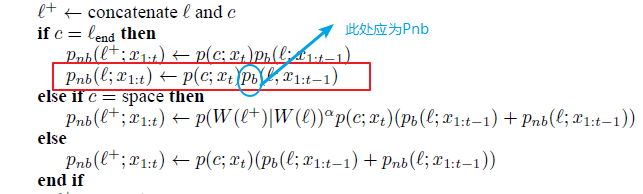
\includegraphics[width=0.6\textwidth]{error-prefix}
  \caption{Prefix Beam Search原论文中算法错误地方 \label{fig:error-prefix}}
\end{figure}

另外原论文中关于这一块的计算步骤写错了,也就是算法中的这一步,如图\ref{fig:error-prefix}。简直坑死个人。

\begin{lstlisting}[language = shell, numbers=left, 
         numberstyle=\tiny,keywordstyle=\color{blue!70},
         commentstyle=\color{red!50!green!50!blue!50},frame=shadowbox,
         rulesepcolor=\color{red!20!green!20!blue!20},basicstyle=\ttfamily]
elif len(l.replace(' ', '')) > 0 and c in (' ', '>'):
  lm_prob = lm(l_plus.strip(' >')) ** alpha
  Pnb[t][l_plus] += lm_prob * ctc[t][c_ix] * (Pb[t - 1][l] + Pnb[t - 1][l])
\end{lstlisting}

那还有可能当前的输出是 ' '(space),也就是说输出是空格或者是结尾,这个时候说明一个完整的词出现了,我们就可以利用语言模型(LM)来对输出进行修正和约束,避免出现毫无意义的结果。那么这个词代入到语言模型中会出现一个概率值,当前候选序列的概率值就通过公式\ref{eqn:with-lm}来计算,从代码中也可以看出来。

\begin{lstlisting}[language = shell, numbers=left, 
         numberstyle=\tiny,keywordstyle=\color{blue!70},
         commentstyle=\color{red!50!green!50!blue!50},frame=shadowbox,
         rulesepcolor=\color{red!20!green!20!blue!20},basicstyle=\ttfamily]
Pnb[t][l_plus] += ctc[t][c_ix] * (Pb[t - 1][l] + Pnb[t - 1][l])
\end{lstlisting}

还有最后一种情况,就是既不是 blank,又不是 space,当前输出标签和候选标签序列的最后一个字母也不一样,这个时候,就直接算出候选标签序列和当前标签的概率乘积就行,候选标签序列也有两种情况:上一个时刻以blank或者以non-blank结尾。综上集中基本的情况都已经讲完了。

\begin{lstlisting}[language = shell, numbers=left, 
         numberstyle=\tiny,keywordstyle=\color{blue!70},
         commentstyle=\color{red!50!green!50!blue!50},frame=shadowbox,
         rulesepcolor=\color{red!20!green!20!blue!20},basicstyle=\ttfamily]
if l_plus not in A_prev:
  Pb[t][l_plus] += ctc[t][-1] * (Pb[t - 1][l_plus] + Pnb[t - 1][l_plus])
  Pnb[t][l_plus] += ctc[t][c_ix] * Pnb[t - 1][l_plus]
\end{lstlisting}

按照原始论文中,还有上面这个公式。也就是说算出来的$l\_plus$不在候选标签序列里面,就会去之前时刻的候选序列里面去找,再利用之前的后续序列概率计算当前的概率值。百度的Deep Speech2代码里面说:这个部分不知道在干啥,还没啥用,所以就给去掉了。

我觉得……也不太好理解……

讲到这儿核心的代码部分已经讲完了,剩下的就是把当前时刻的标签,不管是以blank结尾的还是非blank结尾的综合起来,然后进行排序,根据beam size的大小得到新的候选序列,如此循环往复,直到这个序列输出到了尽头,就可以得到最终的结果啦\~\~\~

完整代码如下:

%%%%%%%%%%%%%%%%%%%%%%%Code for Prefix Beam Search%%%%%%%%%%%%%%%%%%%%%%%%%%%%%%%%%
\begin{lstlisting}[language = python, numbers=left, 
         numberstyle=\tiny,keywordstyle=\color{blue!70},
         commentstyle=\color{red!50!green!50!blue!50},frame=shadowbox,
         rulesepcolor=\color{red!20!green!20!blue!20},basicstyle=\ttfamily]
from collections import defaultdict, Counter
from string import ascii_lowercase
import re
import numpy as np

def prefix_beam_search(ctc, lm=None, k=25, alpha=0.30, beta=5, prune=0.001):
  """
  Performs prefix beam search on the output of a CTC network.

  Args:
    ctc (np.ndarray): The CTC output. Should be a 2D array (timesteps x alphabet_size)
    lm (func): Language model function. Should take as input a string and output a probability.
    k (int): The beam width. Will keep the 'k' most likely candidates at each timestep.
    alpha (float): The language model weight. Should usually be between 0 and 1.
    beta (float): The language model compensation term. The higher the 'alpha', the higher the 'beta'.
    prune (float): Only extend prefixes with chars with an emission probability higher than 'prune'.

  Retruns:
    string: The decoded CTC output.
  """

  lm = (lambda l: 1) if lm is None else lm # if no LM is provided, just set to function returning 1
  W = lambda l: re.findall(r'\w+[\s|>]', l)
  alphabet = list(ascii_lowercase) + [' ', '>', '%']
  F = ctc.shape[1]
  ctc = np.vstack((np.zeros(F), ctc)) # just add an imaginative zero'th step (will make indexing more intuitive)
  T = ctc.shape[0]

  # STEP 1: Initiliazation
  O = ''
  Pb, Pnb = defaultdict(Counter), defaultdict(Counter)
  Pb[0][O] = 1
  Pnb[0][O] = 0
  A_prev = [O]
  # END: STEP 1

  # STEP 2: Iterations and pruning
  for t in range(1, T):
    pruned_alphabet = [alphabet[i] for i in np.where(ctc[t] > prune)[0]]
    for l in A_prev:
      
      if len(l) > 0 and l[-1] == '>':
        Pb[t][l] = Pb[t - 1][l]
        Pnb[t][l] = Pnb[t - 1][l]
        continue  

      for c in pruned_alphabet:
        c_ix = alphabet.index(c)
        # END: STEP 2
        
        # STEP 3: “Extending” with a blank
        if c == '%':
          Pb[t][l] += ctc[t][-1] * (Pb[t - 1][l] + Pnb[t - 1][l])
        # END: STEP 3
        
        # STEP 4: Extending with the end character
        else:
          l_plus = l + c
          if len(l) > 0 and c == l[-1]:
            Pnb[t][l_plus] += ctc[t][c_ix] * Pb[t - 1][l]
            Pnb[t][l] += ctc[t][c_ix] * Pnb[t - 1][l]
        # END: STEP 4

          # STEP 5: Extending with any other non-blank character and LM constraints
          elif len(l.replace(' ', '')) > 0 and c in (' ', '>'):
            lm_prob = lm(l_plus.strip(' >')) ** alpha
            Pnb[t][l_plus] += lm_prob * ctc[t][c_ix] * (Pb[t - 1][l] + Pnb[t - 1][l])
          else:
            Pnb[t][l_plus] += ctc[t][c_ix] * (Pb[t - 1][l] + Pnb[t - 1][l])
          # END: STEP 5

          # STEP 6: Make use of discarded prefixes
          if l_plus not in A_prev:
            Pb[t][l_plus] += ctc[t][-1] * (Pb[t - 1][l_plus] + Pnb[t - 1][l_plus])
            Pnb[t][l_plus] += ctc[t][c_ix] * Pnb[t - 1][l_plus]
          # END: STEP 6

    # STEP 7: Select most probable prefixes
    A_next = Pb[t] + Pnb[t]
    sorter = lambda l: A_next[l] * (len(W(l)) + 1) ** beta
    A_prev = sorted(A_next, key=sorter, reverse=True)[:k]
    # END: STEP 7

  return A_prev[0].strip('>')

\end{lstlisting}

%------------------------------------------------------------------------------
%                                RNN Tranducer 
%------------------------------------------------------------------------------
\section{RNN-Tranducer}

%------------------------------------------------------------------------------
%                                Attention 
%------------------------------------------------------------------------------
\section{Attention}

%------------------------------------------------------------------------------
%                                Transformer 
%------------------------------------------------------------------------------
\section{Transformer}


%------------------------------------------------------------------------------
%                                CNNs 
%------------------------------------------------------------------------------
\section{CNNs}

%------------------------------------------------------------------------------
%                                Mixed Models 
%------------------------------------------------------------------------------
\section{Mixed Models}

\subsection{Self-Attention Transducers for End-to-End Speech Recognition}
这篇论文的作者是田正坤,来自中国科学院自动化所。本论文的主要贡献有:
\begin{enumerate}
  \item 用self-attention模块替代了原来RNN-T中的RNN部分,可以用于并行计算;
  \item 利用 path-aware regularization 帮助SA-T学习对齐;
  \item 使用了chunk-flow机制来进行解码。
\end{enumerate}

\subsubsection{SA-T的基本结构}

\subsubsection{path-aware regularization}

\subsubsection{chunk flow mechanism}

